\begin{figure}[t!]
\centering
    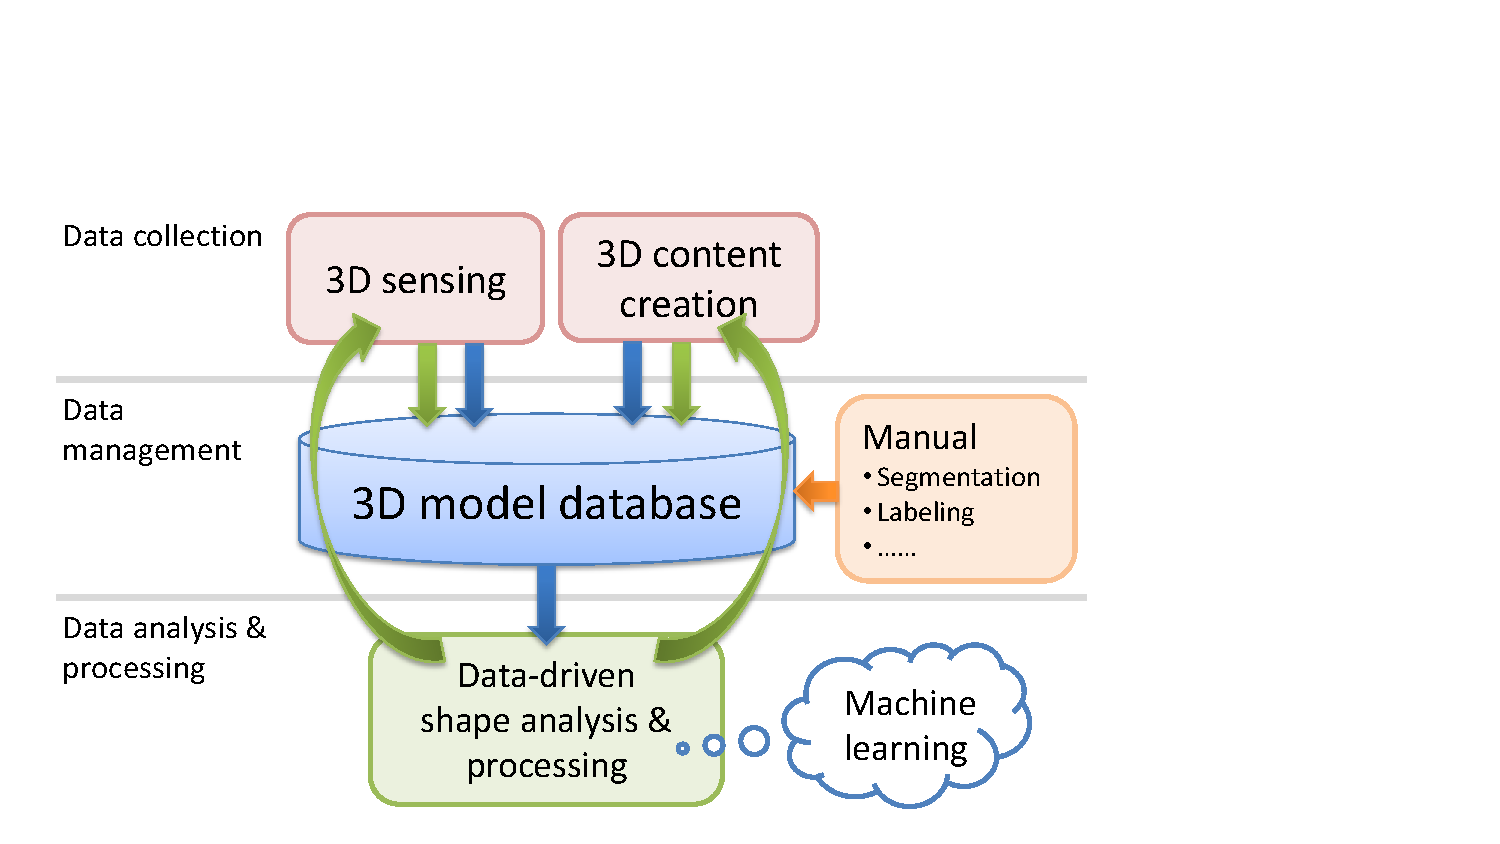
\includegraphics[width=0.99\linewidth]{fig/img/teaser.pdf}
    %\vspace{-.2cm}
    \caption{\rev{Data-driven shape processing and modeling provides a promising solution to the development of ``big 3D data''.
    The two major ways of 3D data generation, 3D sensing and 3D content creation, populate 3D databases with fast growing amount of 3D models.
    The database models are sparsely augmented with manual segmentation and labeling, as well as reasonably
    organized, to support data-driven shape analysis and processing, based on, e.g., machine learning techniques.
    The learned knowledge can in turn support efficient 3D reconstruction and 3D content creation, during which
    the knowledge can be transferred to the newly generated data.
    Such 3D data with semantic information can be included into the database to enrich it and facilitate further data-driven applications.}}
    \label{fig:teaser}
\end{figure}

